\documentclass{article}


% if you need to pass options to natbib, use, e.g.:
%     \PassOptionsToPackage{numbers, compress}{natbib}
% before loading neurips_2022


% ready for submission
% \usepackage{neurips_2022}


% to compile a preprint version, e.g., for submission to arXiv, add add the
% [preprint] option:
%     \usepackage[preprint]{neurips_2022}


% to compile a camera-ready version, add the [final] option, e.g.:
    \usepackage[final]{neurips_2022}


% to avoid loading the natbib package, add option nonatbib:
  %  \usepackage[nonatbib]{neurips_2022}


\usepackage[utf8]{inputenc} % allow utf-8 input
\usepackage[T1]{fontenc}    % use 8-bit T1 fonts
\usepackage{hyperref}       % hyperlinks
\usepackage{url}            % simple URL typesetting
\usepackage{booktabs}       % professional-quality tables
\usepackage{amsfonts}       % blackboard math symbols
\usepackage{nicefrac}       % compact symbols for 1/2, etc.
\usepackage{microtype}      % microtypography
\usepackage{xcolor}         % colors

\definecolor{mygreen}{RGB}{22, 139, 22}
%%%%%%%%%%%%%%%%%%%%%%%%%%%%%%%%%%%%%%%%%%%%%%%%%%%%%%%%%%%%%%%%%%%%%%%%%%%%%%%%%%
% things we added

\usepackage{amsmath}
\usepackage{amssymb}
\usepackage{amsthm}
\usepackage{bbm}
\usepackage{graphicx}
\graphicspath{ {./figures/} }
\newcommand{\RR}{\mathbb{R}}
\newcommand{\PP}{\mathbb{P}}
\newcommand{\cS}{\mathcal{S}}
\newcommand{\cA}{\mathcal{A}}
\newcommand{\cM}{\mathcal{M}}
\bibliographystyle{abbrvnat}


%%%%%%%%%%%%%%%%%%%%%%%%%%%%%%%%%%%%%%%%%%%%%%%%%%%%%%%%%%%%%%%%%%%%%%%%%%%%%%%%%%

\title{Revisiting the Fuzzy Tilling Activation and How to Set its Hyperparameters}


% The \author macro works with any number of authors. There are two commands
% used to separate the names and addresses of multiple authors: \And and \AND.
%
% Using \And between authors leaves it to LaTeX to determine where to break the
% lines. Using \AND forces a line break at that point. So, if LaTeX puts 3 of 4
% authors names on the first line, and the last on the second line, try using
% \AND instead of \And before the third author name.


\author{%
  Muhammad Gohar Javed \\
  Department of Electrical and Computer Engineering \\
  University of Alberta\\
  % Pittsburgh, PA 15213 \\
  \texttt{javed4@ualberta.ca} \\
  % examples of more authors
  \And
  Tian Xiang Du \\
  Department of Computer Science\\
  University of Alberta\\
  \texttt{tdu@ualberta.ca} \\
  \AND
  Amir Bahmani \\
  Department of Computer Science\\
  University of Alberta\\
  \texttt{bahmani1@ualberta.ca} \\
  \And
  Vlad Tkachuk \\
  Department of Computer Science\\
  University of Alberta\\
  \texttt{vtkachuk@ualberta.ca} \\
  % \And
  % Coauthor \\
  % Affiliation \\
  % Address \\
  % \texttt{email} \\
}


\begin{document}


\maketitle


\begin{abstract}
  Sparsity has been shown to improve model performance on decision making problems with non-stationary data, such as online supervised learning and reinforcement learning (RL).
  Sparsity is when a large number of neurons in a neural network are approximately zero.
  The fuzzy tiling activation (FTA) has been proposed to enforce sparsity by design, and has been shown to outperform other activations, such as ReLU and $\tanh$, that do not enforce sparsity.
  However, a difficulty of using the FTA is that it is sensitive to a new \textit{tiling bound} hyperparameter, which currently requires a search to be set effectively.
  In this work we do two things.
  First, we reproduce experiments comparing FTA with ReLU when using deep Q-learning (DQN) on the LunarLander RL environment, showing that indeed, for this environment FTA is no better than ReLU if the tiling bound is not set appropriately.
  Second, we empirically test if simple techniques for normalizing the activation values passed into the FTA cell can remove the need for search when setting the tiling bound.
  Our experiments indicate that normalizing via tanh activation is most effective.


\end{abstract}


\section{Introduction} \label{sec:intro}
Neural networks (NN) have been shown to perform well on several challenging problems \cite{brown2020language,krizhevsky2017imagenet,mnih2013playing,silver2017mastering}
Part of the reason for their success is due to their ability to learn good representations of the input data, which can then be used to effectively generalize.
A representation of an input is defined as the values of all the neurons (except the neurons of the final layer) of the NN when the input is passed into the NN.
The values of all the neurons are commonly called \textit{features}.
Unfortunately, when the NN is trained online (data recieved sequentially), interference can occur between the representations that are learned \cite[]{chandak2019learning,caselles2018continual,madjiheurem2019representation}.
Interference is loosely defined as when a newly learned representation affects the performance of the NN on previously seen data in a negative way (i.e. the old representation becomes worse due to the newly learned one).
A potentially useful intuition for when interference can occur is when the representation for some input $x_1$ is dense (a large number of neurons are non-zero),
since then, if another input $x_2$ is sufficiently different (uncorrelated) from $x_1$, its representation should likely be quite different.
However, in order for a different representation to be learned for $x_2$ the NN will likely have to update the weights that contribute to the representation of $x_1$,
thus making the representation for $x_1$ worse in order to learn a good representation for $x_2$.

A method that has been found to reduce interference, is to enforce sparse representations (a large number of neurons are approximately zero) \cite[]{liu2019,javed2019,rafati2019learning}.
We revisit the example above with inputs $x_1$ and $x_2$.
If the representation for $x_1$ is sparse, then the representation that is learned for $x_2$ can use weights that are unused for the representation of $x_1$,
thus causing no interference between the representations for $x_1$ and $x_2$.
The best way to enforce sparsity is an active topic of research.
A detailed discussion of related works can be found in Section \ref{sec:background}.

One way to enforce sparsity is by design, a method which does this is using a \textit{fuzzy tiling activation} (FTA) \cite[]{pan2019fuzzy}.
FTA is an activation function that can be used at each layer of a NN, similar to ReLU or $\tanh$.
Different from ReLU and $\tanh$ is that FTA has a vector output instead of a scalar output.
FTA takes as input a scalar and outputs a one-hot vector.
The output of FTA can be thought of as mapping a scalar $z \in \RR$ to one of $k$ evenly spaced bins in $\RR^k$.
A critical step to using FTA effectively is setting the tiling bound parameter $u$.
This is because $z$ should be in $[-u, u]$ to work well.
However, just satisfying this is usually not enough for good performance (as one could easily set $u$ very large).
For instance if $u = 10$ and $k = 4$ then the bins would be $[-10, -5), [-5, 0), [0, 5), [5, 10]$
and if $z$ really takes values in $[0,1]$ then it will always map to the same bin (bin $3$ since $[0, 1] \subset [0, 5))$.
Thus, as discussed by \cite[]{pan2019fuzzy}, setting the tiling bound is important; however, no good solution exists for setting it other than performing a search.
The sensitivity to the tiling bound was especially prominant in the work of \cite[]{pan2019fuzzy} when using FTA with a deep Q-network (DQN) \cite[]{mnih2013playing} in the LunarLander RL environment.

As such, in this work we aim to do two things:
\begin{enumerate}
  \item We aim to reproduce the FTA vs ReLU using DQN in LunarLander experiments presented in \cite[]{pan2019fuzzy}, to confirm that indeed FTA is sensitive to the tiling bound in this setting.
  \item Next, we aim to test if the simple technique of normalizing the values (using $\tanh$, or batch norm) passed to FTA can remove the need for tuning the tiling bound parameter in FTA.
\end{enumerate}

Experiments related to the first point are shown in section \ref{sub-sec:reproduc experiments}.

To answer the question in the second point we normalize the values passed into FTA using two methods: passing them into a $\tanh$, using batch norm.
The method of using $tanh$ to normalize the input values was discussed in \cite{pan2019fuzzy}, but not tested.
\cite{pan2019fuzzy} mentioned that using this method might suffer from vanishing gradients, which we hope to confirm from this experiment.
We hypothesis that normalizing the values should solve the need to set tiling bounds using search, since normalizing will ensure that then values passed into FTA are in $[-1, 1]$, thus the tiling bound can always be set to $[-1, 1]$.
Experiments related to the second point are shown in section \ref{sub-sec:normalize experiments}.


\section{Background} \label{sec:background}
Representation learning can influence learning efficiency, positively through generalization but negatively through interference \cite[]{bullinaria1995, iCaRL2016, le2017, liu2019}.
Learned representations using neural networks are especially vulnerable to interference due to aggressive generalization, as updates to one feature’s estimates change the estimates of later features in unexpected ways, degrading model accuracy.
Interference in features learned by neural networks is even worse when trained on temporally correlated data \cite[]{liu2020, bengio2020, zhang2022}

Several authors \cite[]{ghiassian2020,liu2019,javed2019,sutton2019}
have shown that sparse representations can reduce interference in learning feature updates: only a small number of features are active for any given input,
and thus each update is less likely to interfere with the weights of other features. Sparse feature spaces can still be highly expressive and interpretable,
as outputs can be traced to the activation of the most input-discriminative features.
However, learning such sparse representations in the online setting remains an open problem.

Existing strategies to ensure sparsity are to pre-train representations offline using regularizers \cite[]{liu2019} or meta-learning \cite{javed2019},
or online methods using regularizers with replay buffers \cite{sutton2019}. While sparsity regularizers do improve learning,
they often lead to high levels of dead neurons and thus degrades the learned representation over time \cite[]{sutton2019}.
Kernel representations can also provide sparse representations online, but do not scale well to large problems due to its computational complexity \cite[]{pan2019fuzzy}.
Therefore, there is motivation to find a simpler method to ensure sparsity in learned representations that is easy to implement, train, and scale to larger input spaces.

FTA is an approach to achieve sparsity by design,
where an activation function that can be applied to any layer of a neural network provides adjustable sparsity without the need for pre-training or adjustments to the loss function.
The FTA function aggregates inputs of any feature layer into bins with differentiable, overlapping zones. Much like Tile Coding \cite[]{tilecoding},
FTA allows learning to be discriminative between different input values through binning, but unlike Tile Coding,
FTA maintains input generalization through learning activations within the differentiable regions between bins.
When applied to DQN and Deep Deterministic Policy Gradient (DDPG) \cite[]{ddpg},
FTA has been empirically shown to improve agent performance for both discrete and continuous control environments,
often outperforming activations like ReLU and Tanh \cite[]{pan2019fuzzy}. Furthermore, FTA-applied networks can often perform better without target networks,
circumventing the sample inefficiency problem inherent in their use \cite[]{pan2019fuzzy}.
A recent study by \cite{nnrep} on transferring learned representations to networks performing auxiliary tasks found that FTA-based representations
transferred better and more consistently than ReLU-based representations for less similar tasks.

\section{Preliminaries} \label{sec:prelims}
In this section we introduce the Fuzzy Tiling Activation (FTA) and formally define the RL setting.

\subsection{Fuzzy Tiling Activation}
First we introduce the simpler \textit{tiling activation} (TA) and then extend it to the FTA.
A TA is a function $\phi: \RR \to \RR^k$, which expects inputs $z \in [-u, u]$ and maps them to one-hot vectors (standard basis) in $\RR^k$.
The $[-u, u]$ is referred to as the tiling bound.
For example, if $u=10$ and $k=4$, then any $z \in [-10,-5)$ would be mapped to $(1, 0 ,0, 0) \in \RR^k$, any $z \in [-5, 0)$ would be mapped to $(0, 1, 0, 0)$, any $z \in [0, 5)$ would be mapped to $(0, 0, 1, 0)$, and any $z \in [5, 10]$ would be mapped to $(0, 0, 0, 1)$.
\cite{pan2019fuzzy} show that the TA can be implemented efficientely as follows.
Assume you want evenly spaced bins of size $\delta > 0$, and $k = 2 u/ \delta$, where WLOG $u$ was chosen such that it is divisable by $\delta$.
Define the tiling vector
$$\mathbf{c} = (-u, -u + \delta, l + 2 \delta, \dots, u - 2 \delta, u - \delta) \in \RR^k$$
Then the TA can be defined as
$$\phi(z) = \mathbbm{1} - I_+(\max(\mathbf{c} - z\mathbbm{1}, 0) + \max((z -\delta)\mathbbm{1} - \mathbf{c}, 0))$$
where $\mathbbm{1} \in \RR^k$, and $I_+(\cdot)$ is an indicator function which returns 1 if the input is positive and zero otherwise, and is applied element wise to vectors.

An issue with the TA is that it has zero derivative almost everywhere.
In order to solve this issue \cite{pan2019fuzzy} proposed modifying the TA for a fuzzy tiling activation (FTA).
The FTA can be implemented as follows.
Define a fuzzy version of the indicator function as
$$I_{\eta, +} = I_+(\eta -x)x + I_+(x - \eta)$$
where $\eta \ge 0$.
Then the FTA can be defined as
$$\phi_\eta(z) = \mathbbm{1} - I_{\eta, +} (\max(\mathbf{c} - z \mathbbm{1}) + \max((z-\delta)\mathbbm{1} - \mathbf{c}, 0)).$$
where $I_{\eta, +}$ is applied element wise to vectors
The reason for the use of fuzzy in the name of FTA can be understood from the definition of $I_{\eta, +}$.
The term $I_+(\eta -x)$ is $1$ when $x < \eta$, while when $x > \eta$, $I_+(x - \eta)$ is $1$.
Thus, when $x < \eta$ we have that $I_{\eta ,+}$ evaluates to $x$, giving a smoother (fuzzy) indicator function.
Notice, that this means for $x < \eta$ the derivative is non-zero, allowing us to use backpropagation to train out networks.
Also, when $\eta = 0$ the original indicator function $I_+$ can be recovered.

\subsection{ReLU Activation}
We will be comparing FTA to the rectified linear activation (ReLU) later
% , and will be using $\tanh$ to help improve the performance of FTA in Section 4.2.
Thus we formally introduce it now.
ReLU is defined as the positive part of its argument. Formally
$$\phi(z) = \max(0, z)$$.
% While $tanh$ is defined Assume

\subsection{Reinforcement Learning} \label{sub-sec:reinforcement}
The reinforcement learning (RL) setting can be formulated as an markov decision process (MDP).
Formally an MDP is characterized by the tuple $(\cS, \cA, \PP, R, \gamma)$, where $\cS$ is that state space, $\cA$ is the action space,
$\PP$ is the transition probability kernel, $R: \cS \times \cA \times \cS \to \RR$ is the reward function, and $\gamma \in [0, 1]$ is the discount factor.
A policy $\pi: \cS \to \cM_1$ is a map from states to distributions over actions, where $\cM_1$ is the set of all probability measures over actions $\cA$.
Then, an agent (policy) interacts with an MDP as follows.
At each time step $t \in 1, 2 \cdots$ the agent observes a state $s_t \in \cS$.
The agent takes an action according to its policy $a_t \sim \pi(s_t)$.
The agent then transits to its next state according to $s_{t+1} \sim \PP(s_t, a_t)$, and recieves a reward $R(s_t, a_t, s_{t+1})$.

An action value function under policy $\pi$ is defined as
$$Q_\pi(s, a) := \mathbf{E}[G_t|S_t =s, A_t=a; A_{t+1: \infty} \sim \pi]$$
where $G_t := \sum_{t=0}^\infty \gamma^t R(s_t, a_t, s_{t+1})$ is the return.
The goal of the agent is maximize its expected reward from each state in $\cS$.

\subsection{Deep Q-Learning} \label{sub-sec:dqn}
In our experiments, we use Deep Q-Learning (DQN) \cite[]{mnih2013playing}.
As explained in section \ref{sub-sec:reinforcement}, the goal of the agent is to interact with the environment in a way that maximizes its expected reward.
The optimial action value function is defined as
$$Q^*(s, a) = \mathbf \max_{\pi} Q_\pi(s, a)$$

In Q-Learning the action value function is iteratively updated by using the following (Bellman) equation to converge to the optimal action value function
$$Q_{t+1}(s, a) = \mathbf{E}[R(s_t, a_t, s_{t+1}) + \gamma \max_{a_{t+1} \in \cA} Q_t(s_{t+1}, a_{t+1})|S_t =s, A_t=a, S_{t+1}=s_{t+1}]$$
This converges to optimal action value function, $Q_t \rightarrow Q^*, t \rightarrow \infty$.
A NN is used as a function approximator with weights $\theta$ to estimate an action value function, $Q(s, a; \theta)$
The NN is trained by minimizing the following loss function at each time step $t$
$$L_t(\theta_t) = \mathbf{E}_{s, a\sim \rho(.)}\big[(y_t - Q(s, a; \theta_t))^2\big],$$
where $y_t = \mathbf{E}_{s^\prime\sim\varepsilon}[r + \gamma \max_{a^\prime}Q(s^\prime, a^\prime; \theta_{i-1}) | s, a]$.
The loss is computed by taking the expectation over the state-action pairs, $s, a$, that are sampled from the current $\mathit{behavior\ policy}$ $\rho(s, a)$.
The expected value of the squared difference between the target value $y_i$ and the predicted action-value $Q(s, a; \theta_i)$ is then computed.
The target value $y_i$ is a measure of the long-term rewards that can be obtained by taking a given action in a given state.
It is computed by taking the expected value of the sum of the immediate reward $r$ and the discounted future rewards $\gamma \max_{a^\prime}Q(s^\prime, a^\prime; \theta_{i-1})$, where $s^\prime$ is a future state that is obtained by taking action $a$ in state $s$, and $a^\prime$ is the action that maximizes the expected future rewards.
The expectation is taken over the distribution of future states $s^\prime$ obtained by sampling from the environment with some probability $\varepsilon$.

Agent's experience at each timestep is stored into a $replay\ memory$.
A random minibatch of expriences are samepled randomly from this memory to calculate the loss function, and the neural network is trained by performing a gradient descent on the loss function.


\section{Experiments} \label{sec:experiments}
The LunarLander environment, from OpenAI Gym \cite[]{brockman2016gym} is a trajectory rocket optimization problem, where the goal is to land a moon lander on a landing pad.
The state space of the environment $\cS$ is compromised of 8 attributes; $x$ and $y$ coordinates, $v_x$ and $v_y$ horizontal and vertical velocities, $\theta$ and $v_\theta$ angle and angular velocity, and 2 booleans to show if the left or right leg is touching the ground. At each timestep $t$ the action space $\cA(s_t) = \tt\{do\ nothing,\ fire\ left\ engine,\ fire\ main\ engine,\ fire\ right\ engine\}$. The rewards for landing on the landing pad is between 100 to 140 points, with an additional 100 points if it stops on it, hence a solved episode is +200 points. Firing the main engine has -0.3 and the side engines -0.03 points penalty, and the lander gets -100 points if it crashes. In the event that the agent crashes, leaves the viewport, or remains stationary without touching another body, the episode will terminate.

The CartPole environment is a classic control problem from the OpenAI Gym \cite[]{brockman2016gym} where a pole is attached to a cart that can move along a frictionless track. The goal is to balance the pole by moving the cart back and forth so that it stays upright. The state of the environment is represented by four values: the position and velocity of the cart, and the angle and angular velocity of the pole. The goal of the agent is to balance the pole by moving the cart to left or right. Hence, at each timestep $t$ the action space $\cA(s_t) = \tt\{move\ left,\ move\ right\}$. The Reward for each timestep is +1 and the environment is considered solved if the pole remains upright for a certain number of time steps, without falling over or the cart moving too far from the center of the track.


\subsection{Reproducibility Experiment} \label{sub-sec:reproduc experiments}
Following the same settings as in \cite{pan2019fuzzy}, we use a two-layer neural network with different acivation function in the last hidden layer as the main difference. For DQN and DQN-Large, we use ReLU activation function in all the layers, with the exception of the last layer which is linear.
Since DQN with FTA activation function expands the number of features, its last hidden layer is $k = (l-u)/\delta$ times bigger than the DQN, Hence we use DQN-Large with the last hidden layer of the same size of DQN-FTA with and without the target network.

For DQN-FTA in the last layer we set $[l, u] = [-20, 20]$ and $\eta = \delta = 2.0$, hence $k = 40/2 = 20$.


\begin{figure}[h]
    \centering
    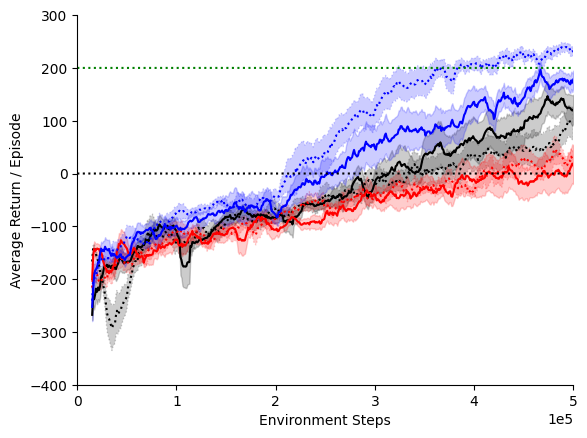
\includegraphics[height=4cm]{ftavrelu.png}
    \caption{Evaluation learning curves of {\bf DQN-FTA(black)}, {\textcolor{red} {\bf DQN(red)}} and {\textcolor{blue} {\bf DQN-Large(blue)} }. The {\bf dotted} line shows the algorithms trained with target network. The results are averaged over 10 runs, with shaded area showing the standard error.}
    \label{fig:ftavrelu}
\end{figure}



In figure \ref{fig:ftavrelu}, we observe that, while DQN-FTA with and without the target network performs slightly better than DQN, DQN-Large outperforms both DQN and DQN-FTA.

To show the sensitivity of DQN-FTA to the tiling bounds, we repeat the experiment for DQN-FTA only, with different values of $u \in \{0.1,1,10,50,100\}, l = -u$ with different number of tiles $k \in \{16, 24, 128\}$ for each tiling bounds.

\begin{figure}[h]
    \centering
    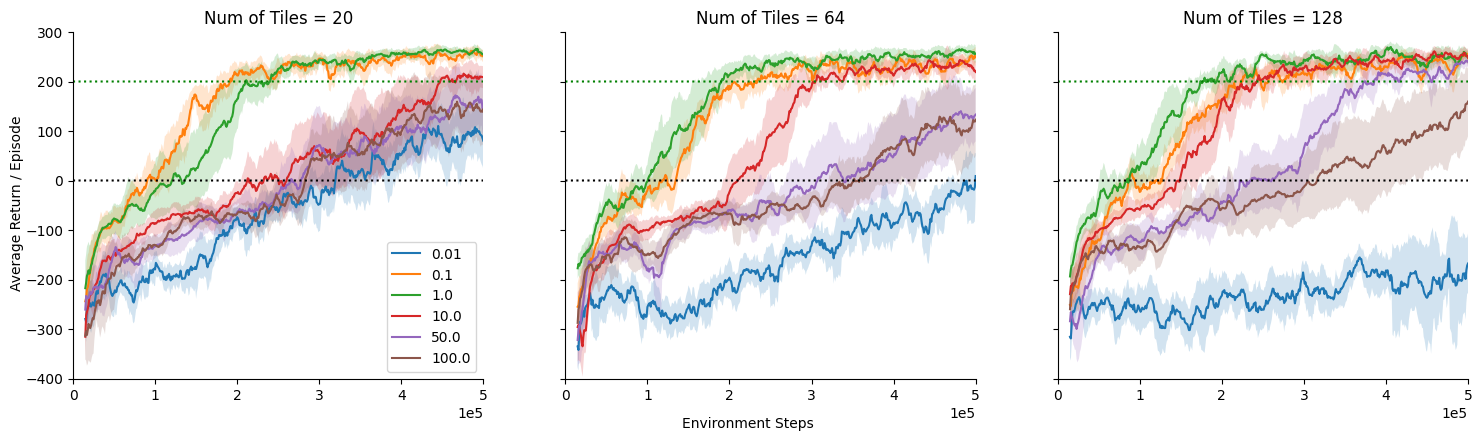
\includegraphics[height=4cm]{sweepfta.png}
    \caption{Evaluation learning curves of DQN-FTA using different values of tiling bounds: $u \in \{0.1, 1, 10, 50, 100\}, l = -u$, with different number of tiles $k \in \{16, 64, 128\}$. The results are averaged over 10 runs.}
    \label{fig:sweepfta}
\end{figure}

Figure \ref{fig:sweepfta} depicts the results of the experiment.
It can be seen that DQN-FTA in LunarLander performs the best, when we set $u$ to a reasonably small value (approximately $u = 1$).
However, it performs poorly when it is set too large ($u=10, 50, 100$) or small ($u=0.01$).
With $u \in \{10, 50, 100\}$, performance improves by increasing the number of tiles $k$, but it gets worse when $u$ is very small.
The improved performance when the number of tiles $k$ is increased can be understood by looking at the case when $u=10$ and $k=128$.
Notice that $u=10$ is $10$ times larger than $u=1$ and $k=128$ is approximately $10$ times larger than $k=16$.
Thus, for the range $[-1, 1]$ there will be approximately the same number of bins when $u=10, k=128$ as when $u=1, k=16$.
This explanation explains why the green line ($u=1$) when $k=16$ is approximately the same as the red line ($u=10$) when $k=128$.

\begin{figure}[h]
    \centering
    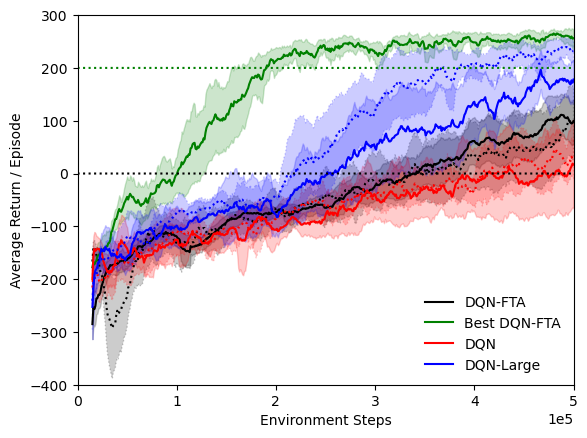
\includegraphics[height=4cm]{bestfta.png}
    \caption{Evaluation learning curves of {\bf DQN-FTA(black) ($u=20, k = 40$)}, {\textcolor{red} {\bf DQN(red)}},  {\textcolor{blue} {\bf DQN-Large(blue)}} and {\textcolor{mygreen} {\bf DQN-FTA(green)}($u=1, k=64$)}. The {\bf dotted} line shows the algorithms trained with target network.}
    \label{fig:bestfta}
\end{figure}

We found FTA sensitive to the tiling bound ($u$), hence only when choosing the the right value of $u$ we observed that it outperforms both DQN and DQN-Large.
We found that the best value $u=1$ for DQN-FTA without a target network was $u=1$
Figure \ref{fig:bestfta} shows a plot of the above described DQN-FTA network compared to the untuned DQN-FTA ($u=20$) and DQN using ReLU activation instead of FTA.
The clearly indicates that when the value of $u$ is set appropriately, DQN-FTA can outperform DQN with ReLU activation.

\subsection{Normalizing Experiment} \label{sub-sec:normalize experiments}
% Explain how we plan to normalize the activation value going into FTA (i.e. $z = \tanh(X w)$).
% I think we can leave this as TODO for final report.
In our experiments, detailed in section \ref{sub-sec:reproduc experiments}, it can be observed that the performance of FTA is quite sensitive to the tiling bound $[-u, u]$.
This reinforces the observation made in \cite{pan2019fuzzy}.
In figure \ref{fig:sweepfta} we can see that the best performance on LunarLander was achieved with $u=1$, and it got worse as we increased or decreased $u$.
It can be inferred intuitively, that for a small value of $u$, many inputs to FTA may be out of its range providing zero gradients.
On the other hand, for a large value of $u$, many inputs may activate the same tile.
Both resulting in many dead neurons and increasing interference.
This means there is a specific value of $u$ which would work best for any specific environment.
Since its not straightforward to observe the range of outputs from a Neural Network layer, $u$ can not be set mathematically.
It has to be tuned manually by sweeping over a range of values in multiple experiments, which increases the cost of a project.

We hypothesize that if the inputs to FTA were scaled to a certain range, the performance would be less sensitive to the tiling bounds.
We try two different methodologies to achieve this.
First, using a Batch Normalization \cite[]{ioffe2015batch} layer before FTA.
Second, using a $tanh$ activation layer before FTA.

Batch Normalization scales its input $x$ to a learned mean $\beta$ and variance $\gamma$.
It is defined as
\begin{equation}
    y = \frac{x-E[x]}{\sqrt{Var[x] + \epsilon}} * \gamma + \beta
    \label{eq:batchnorm}
\end{equation}
By using a Batch Norm layer before FTA, we expect it to learn the best $\gamma$ and $\beta$ for any particular tiling bound of FTA.

On the other hand, $\tanh$ is an activation function which maps the input to a continuous range of values between -1 and 1.
The larger the input, the closer the output is to 1 and the smaller the input, the closer the output is to -1.
This range of outputs can be controlled by multiplying them with a scalar.
It is defined as
 \begin{equation}
    y = \frac{e^x-e^{-x}}{e^x+e^{-x}}
    \label{eq:tanh}
 \end{equation}
The motivation behind using $tanh$ is to control the range of inputs to FTA, so that a standard tiling bound of $u = -l = 1$ would work in every case.

To test these hypothesis, we run two experiments each with $tanh$ and Batch Norm as the layer preceding FTA on Lunar Lander.
One, with the best performing FTA tiling bounds and two, with the worst performing FTA tiling bounds.
All other parameters and configurations are kept the same as those in section \ref{sub-sec:reproduc experiments}.
Figure \ref{fig:bnvtanh} shows the evaluation learning curves plotting episodic return versus environment time steps for all four of these experiments.

\begin{figure}[h]
    \centering
    \includegraphics[width=3cm]{example-image-a}
    \caption{Evaluation learning curves plotting episodic return versus environment time steps for Batch Norm and $tanh$ as layers preceding FTA.}
    \label{fig:bnvtanh}
\end{figure}


\section{Discussion} \label{sec:discussion}
In this paper, we investigate the properties of FTA through empirical experimentation as an extension to the original FTA paper by \cite[]{pan2019fuzzy}.
We first reproduced the learning curve evaluation for DQN-FTA, DQN, and DQN-Large in LunarLander, and found similar trends.
When comparing the untuned FTA agent ($u = 20$) against the tuned ReLU agents, we found that FTA and DQN-Large reached higher average returns
by $5\times10^5$ time steps than \cite{pan2019fuzzy}. It is currently unknown as to why our FTA and DQN-Large implementations perform better than the original paper.
There are many potential reasons: stochasticity in our runs and initialization, our specific seeds used to evaluate performance, or even the implementation framework
(we used PyTorch while \cite{pan2019fuzzy} used TensorFlow) could all influence the empirical outcome of experiments.
While we only average over 10 runs compared to the 20 performed in the original paper, this should not have contributed to the performance discrepancy
given our low standard error between runs. We will contact the original author to address any implementation differences,
but further investigation into the plausible causes and further experimentation are required.

Our second experiment reproduces the bound sensitivity experiment comparing FTA with different tiling bounds,
but also across different numbers of tiles. Our results share the conclusion that moderately small values for $u$ ($u \in {0.1, 1}$)
perform better than the extremes ($u \in {0.01, 10, 50, 100}$) \cite[]{pan2019fuzzy}. We also find that increasing the number of tiles
improves the performance of larger tiling bounds ($u \in {50, 100}$) while an extremely small $u$ gets worse ($u = 0.01$). This is expected,
as increasing the number of tiles given a large tiling bound reduces $\delta$, thereby reducing interference between bins. In addition,
increasing the number of tiles given an extremely small tiling bound greatly increases $delta$ and results in high interference between bins.

To address the bound selection problem, we design normalizing experiments using $tanh$ activation and batch normalization.
\cite{pan2019fuzzy} mention that $tanh$ would not be an effective strategy for ensuring $z \in [l,u]$ given the gradient vanishing problem,
so we will provide empirical data to evaluate this hypothesis. With a principle focus of FTA being its ease of use,
we propose using batch normalization to automatically bound $z \in [l,u]$ without additional tuning.

Lastly, we will reproduce the learning curves comparing FTA against ReLU for Acrobot, MountainCar, and Cartpole,
to investigate if our performance discrepancy exists in other environments.


\newpage
\bibliography{references}

\end{document}
